\documentclass{article}
\usepackage{bigstrut}
\usepackage{adjustbox}
\usepackage{graphicx}^^M
\graphicspath{ {images/} }
\usepackage[T1]{fontenc}
\usepackage{float}

\usepackage[english]{babel}
\usepackage[utf8]{inputenc}
\usepackage{indentfirst}

\addtolength{\oddsidemargin}{-.875in}
\addtolength{\evensidemargin}{-.875in}
\addtolength{\textwidth}{1.75in}
\addtolength{\textheight}{1in}

\usepackage{hyperref}
\hypersetup{
    colorlinks=true,
    linkcolor=blue,
    filecolor=magenta,      
    urlcolor=cyan,
}

%-----ADDING FIGURES------
%\begin{figure}[h]
%\begin{center}
%\includegraphics[width=\textwidth]{IMAGE_NAME_HERE}
%\caption{CAPTION_HERE}
%\end{center}
%\end{figure}

%-----ADDING TABLES-------
%\begin{table}[h]
%\begin{center}
%\begin{tabular}{c|c|c|c|c}
%& Butterworth & Chebyshev & Linkwitz-Riley & Bessel\\
%\hline
%Passband Accuracy & 10 & 4 & 6 & 9\\
%\hline
%Filter Slope & 7 & 10 & 5 & 6\\
%\hline
%Impulse Response & 5 & 7 & 10 & 3\\
%\hline
%Popularity in Crossover Filters & 3 & 3 & 7 & 3\\
%\hline
%Total & 25 & 24 & 28 & 21\\
%\hline
%Rank & 2 & 3 & 1 & 4\\
%\end{tabular}
%\caption{ADD CAPTION HERE}
%\end{center}
%\end{table}

%-----ADDING IMAGES-----
%\begin{center}
%\includegraphics[width=400px]{Image_NAME_HERE}
%\end{center}


\begin{document}
\title{Sanside Technology}
\begin{titlepage}
    
\includegraphics[width = 150px]{images/SansideLogo.png}
    \hfill
    \hrule
    \vspace{2cm}
    \centering
	{\scshape\LARGE Sanside Technology Facebook Integration v2.0\par}
	\vspace{0.5cm}
	{\scshape Marcin Wisniowski: Product Development Intern \par}
    \vspace{2cm}
    \begin{center}
    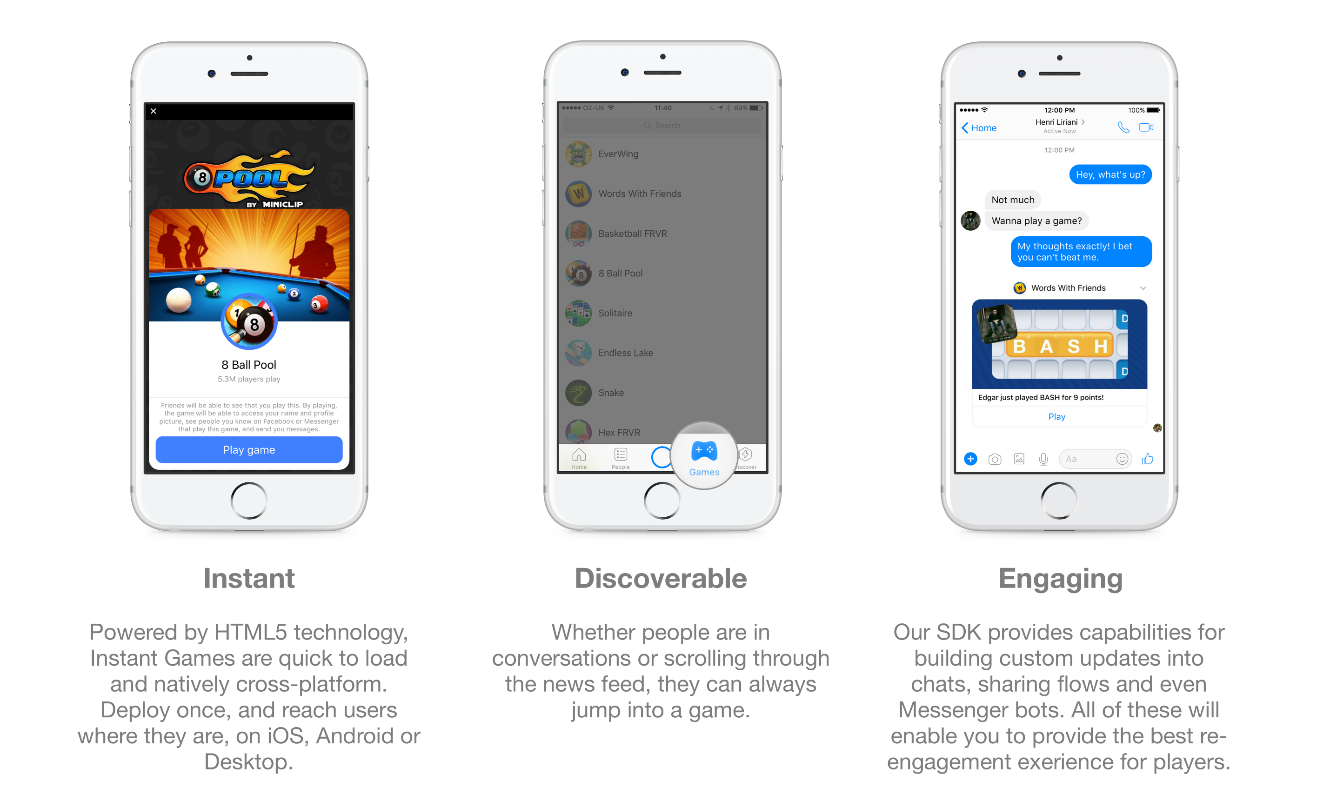
\includegraphics[width = 400px]{images/Facebook.png}
    \end{center}
    \vspace{0.5cm}
    {\scshape A definitive guide to integrating \textbf{Facebook Instant Games} with pre-made HTML5 mobile creations}
\end{titlepage}

\pagenumbering{roman}
\section{Abstract}
Facebook integration is an important step to successfully expand the company's market from local Chinese applications to the global scale. Therefore, being able to adapt pre-made games into a Facebook Instant Games format is relevant in globalizing the production of the HuHuGame division. This document should be used for learning and also referencing necessary information to turn an HTML5 game into a Facebook Instant Game. By the end of the document, the reader should be able to:
\begin{enumerate}
\item Integrate the Facebook SDK into the game files
\item Create an application slot to insert the game into as a Facebook Developer
\item Traverse around the Facebook Business pages
\item Upload and update your game with new versions
\item Insert advertisements into the game
\item Use Facebook Analytics to gain data about your game
\item Send the game into review to be pushed towards the open market
\end{enumerate}

\tableofcontents

\newpage
\pagenumbering{arabic}

\section{Facebook SDK Integration}
\subsection{Inserting the SDK}
The first step in integrating your mobile game with Facebook is to insert the Facebook SDK into your index.html file in order to load up the Facebook Instant Games SDK. This is done by inserting this line of code. It should be the first piece of code after the <body> tag:

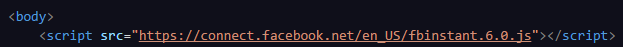
\includegraphics[]{FacebookIndex.png}


Then, in order to be able to use Facebook's pre-made functions across any file, the SDK must be loaded into the egretProperties.json file. This allows the Egret Engine to use the function names within any javascript or typescript file.

\begin{center}
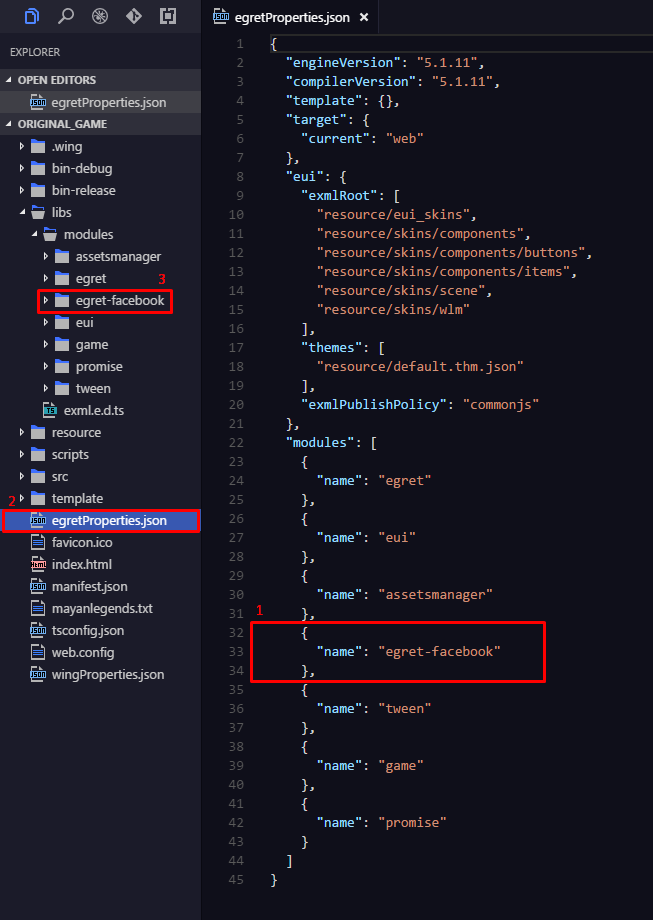
\includegraphics[width = 275px]{images/FacebookSDK.png}
\end{center}

\begin{center}
1. The code that needs to be added to the file \par
2. The file location that it needs to be added to \par
3. The folder that is created after the project is built correctly \par
\end{center}

\newpage

\subsection{Instant Games API Functions}
After the above code is added to the game, FBInstant functions can be used across any file to call functions and get information. The following link shows the entire library of functions that can be used in the future.

\vspace{.5cm}
\href{https://developers.facebook.com/docs/games/instant-games/sdk/fbinstant6.1}{Facebook Instant Games API Reference 6.1}
\vspace{.5cm}

We will focus on three in particular:

FBInstant.initializeAsync() | FBInstant.setLoadingProgress() | FBInstant.startGameAsync()

\subsubsection{FBInstant.initializeAsync()}
This function initializes the SDK, in order for it to work. It is necessary to put this function before any other FBInstant functions for them to work.

\subsubsection{FBInstant.setLoadingProgress()}
When starting up a Messenger game, Facebook integrates its own loading system to use. To allow it to show correctly, the programmer should update this function with each asset as it is loaded, from a percentage of total assets. This way the user knows what percentage of the game is loaded and when it is fully loaded in order to play it.

\subsubsection{FBInstant.startGameAsync()}
This function tells Messenger to remove the loading screen from the main interface and load up the game. In the case of egret, this function should come right before the GameScene is created.

\subsubsection{Example}
\begin{center}
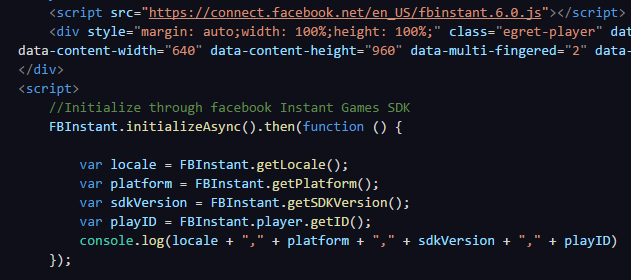
\includegraphics[width = \textwidth]{images/FacebookInitialize.png} 

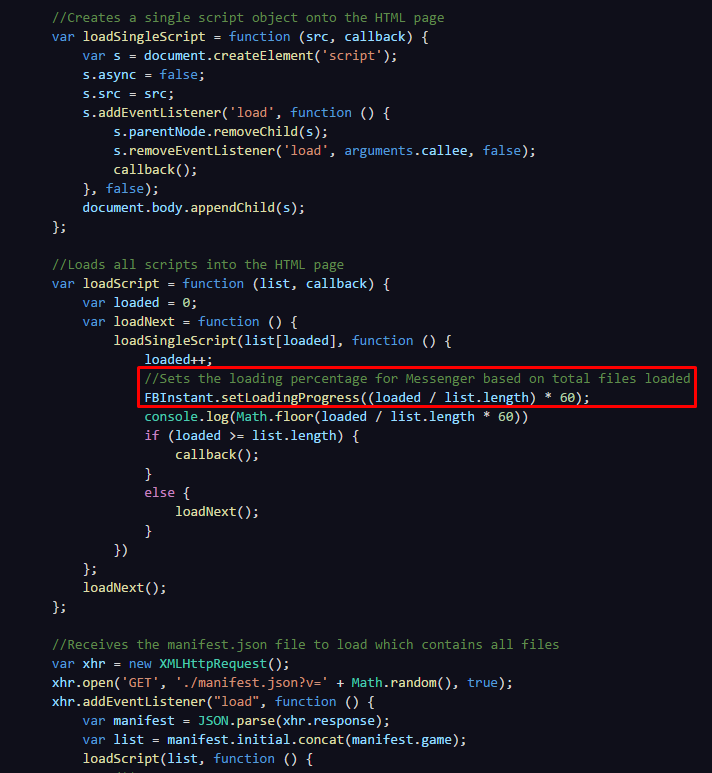
\includegraphics[width = \textwidth]{images/FacebookLoading.png} Index.html

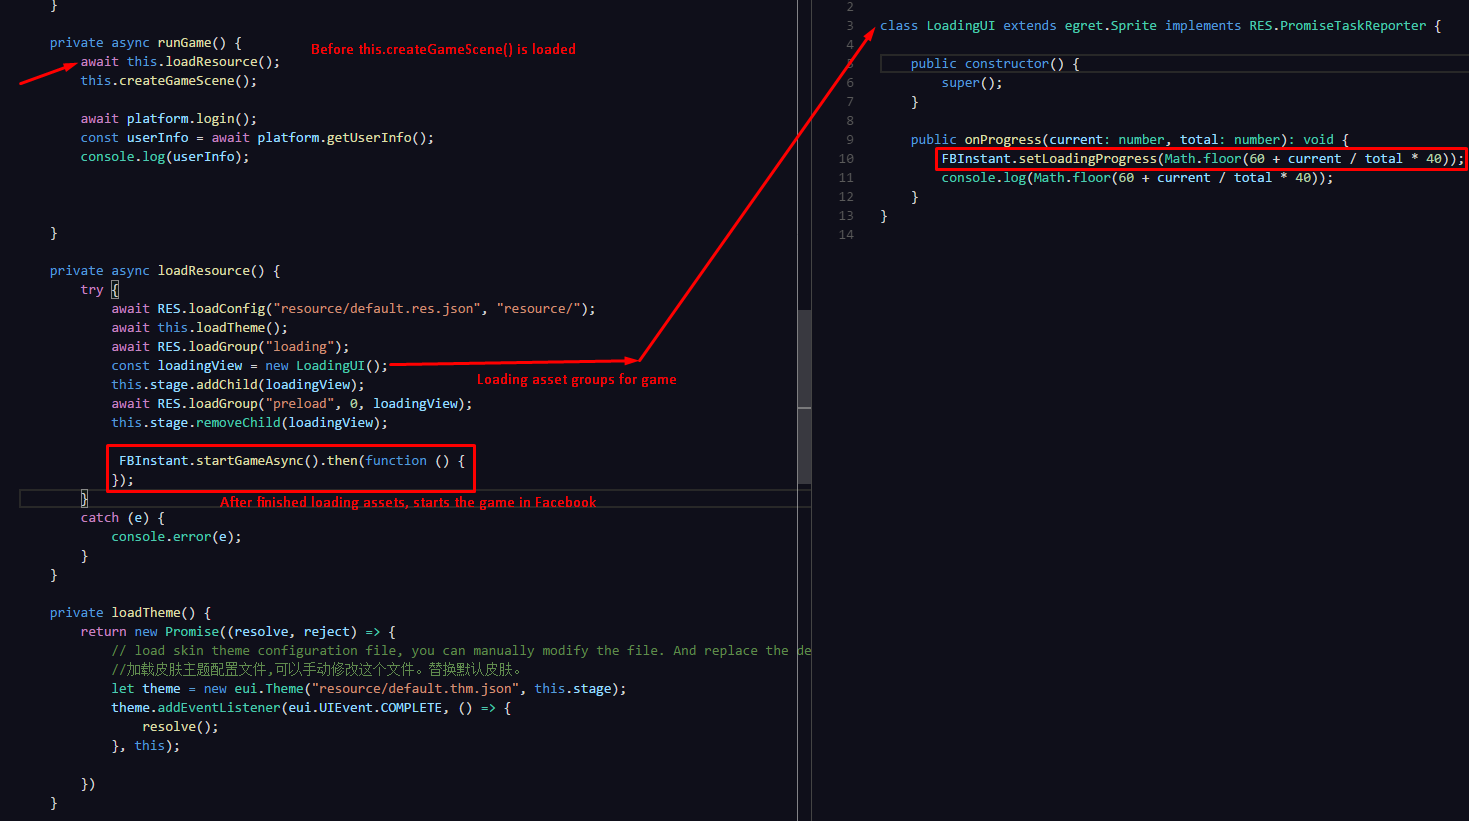
\includegraphics[width = \textwidth]{images/FacebookInitialize2.png} Main.ts
\end{center}

\section{Facebook Application Creation Process}
After the game is set up and ready to be uploaded onto the Facebook platform, an application slot must be created for it within the Facebook Business website. Follow this guide for a brief explanation on how to navigate around, however the website itself can be accessed in Chinese for easier navigating.

\vspace{.2cm}
\begin{center}
\href{https://business.facebook.com}{Facebook Business Website}
\end{center}

\begin{table}[h]
\begin{center}
\begin{tabular}{c|c}
Username: \hspace{1cm} & sansidekeji@outlook.com \\
Password: \hspace{1cm} & Maxing2018yes 
\end{tabular}
\caption{Facebook Login Credentials}
\end{center}
\end{table}

\subsection{Navigation}
After logging into the website, locate the App Dashboard menu under the options. Here you can see a page for all of your Instant Games applications on one screen and click on each for more information about them.

\begin{center}

\includegraphics[width = \textwidth]{images/AppDashboardPage.png}

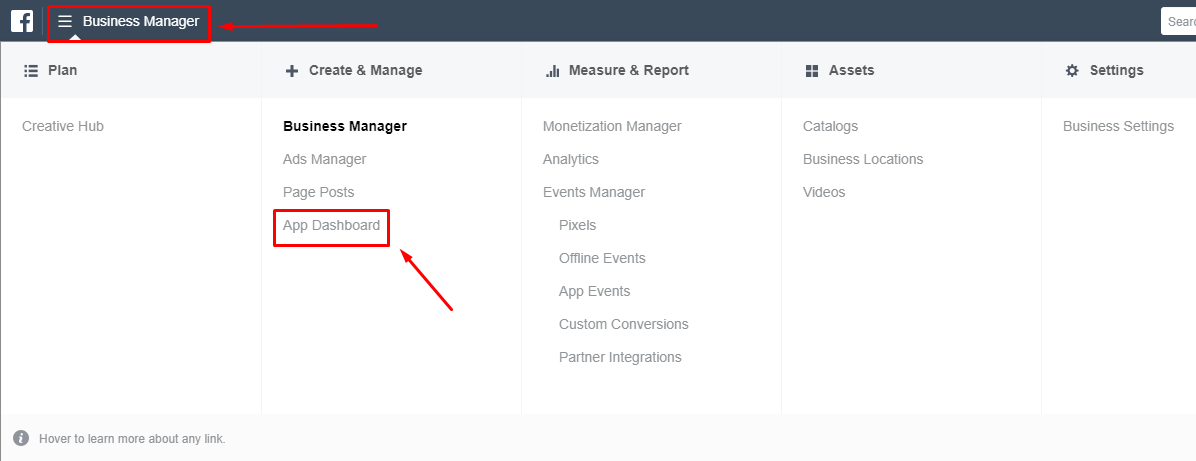
\includegraphics[width = \textwidth]{images/AppDashboardEnglish.png} 
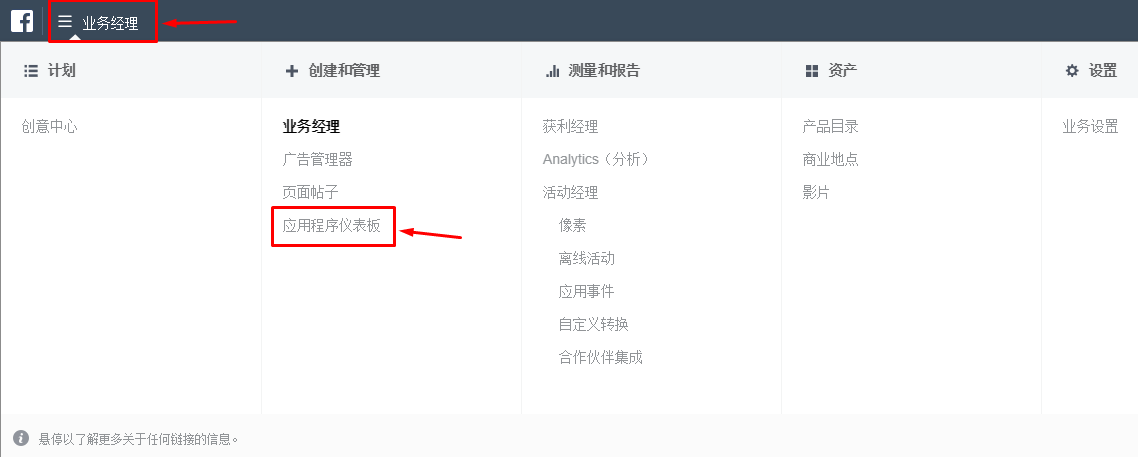
\includegraphics[width = \textwidth]{images/AppDashboardChinese.png}
\end{center}

\newpage

\subsection{Creating the Game}\hypertarget{creatinggame}
When creating a new application, make sure to select "Audience Network" in order to be able to show advertisements and "Instant Games" to make it compatible with Facebook Instant Games. The other Product Options can also be added as needed including analytics, App Center, and Instagram API.

\begin{center}
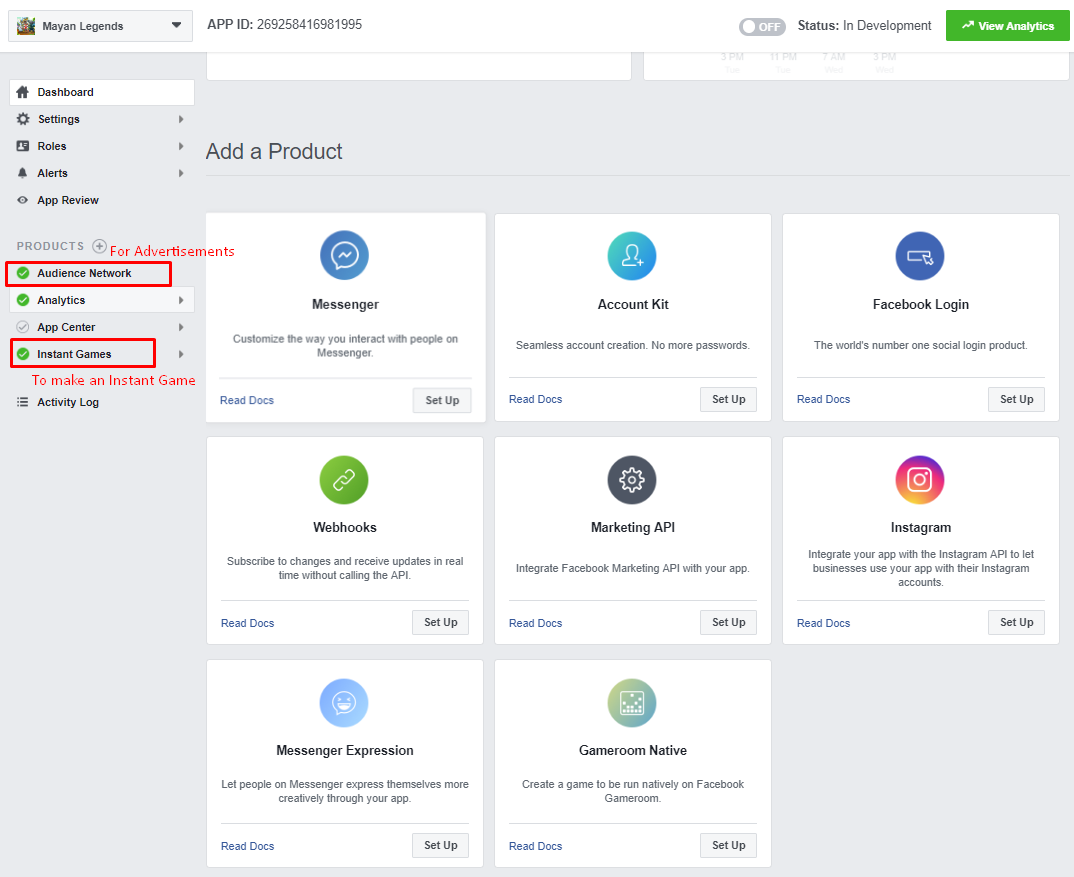
\includegraphics[width = 350px]{images/ProductOptions.png}
\end{center}

\subsection{Uploading the Game}
Finally, in order to upload your game, after adding the Instant Games product, go to Web Hosting and upload your game folder. In order to upload, the file must be zipped (.zip). Then, once it uploads and is scanned by Facebook it can be pushed to production by click on the star.

\begin{center}
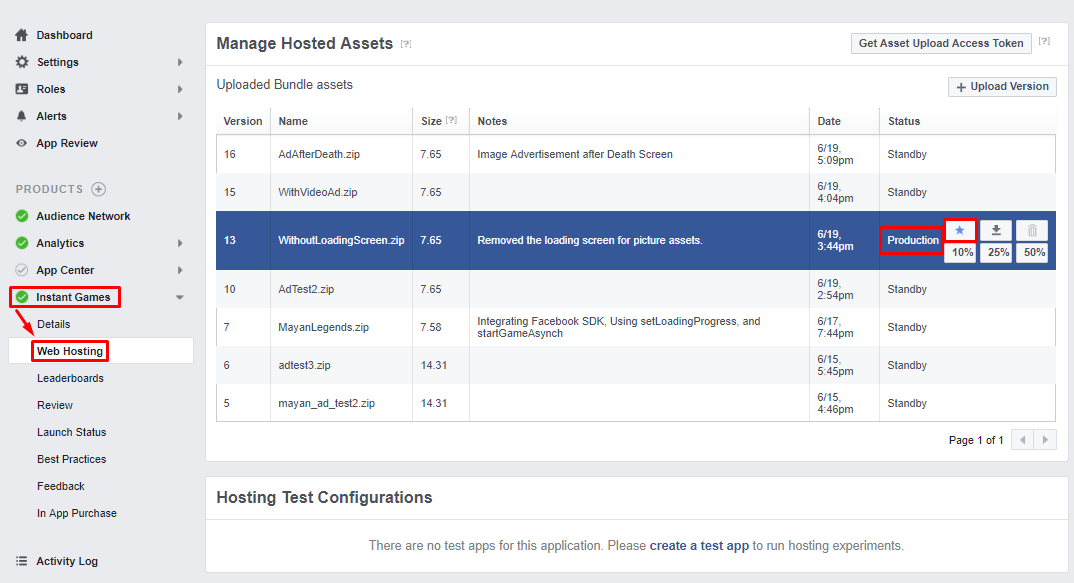
\includegraphics[width = 350px]{images/HostingScreen.png}
\end{center}

\section{Advertisements}
In order to make applications profitable, advertisements can be added to the game. Facebook allows developers to use its database of advertisements to show the user under the condition that the application gets approved by Facebook to be able to show advertisements. After a game is ready to be released, it should be sent to Facebook for approval to place into the market for advertisements to show up in the published game. 

\subsection{Audience Network}
This database of advertisements is called the "Audience Network". Therefore, in order to have ads in your game, your game must be set up with an audience network. In order to create an advertisement placement in your game, your game must first be connected to an Audience Network when made \hyperlink{creatinggame}{(see Creating the Game)}.

\begin{center}
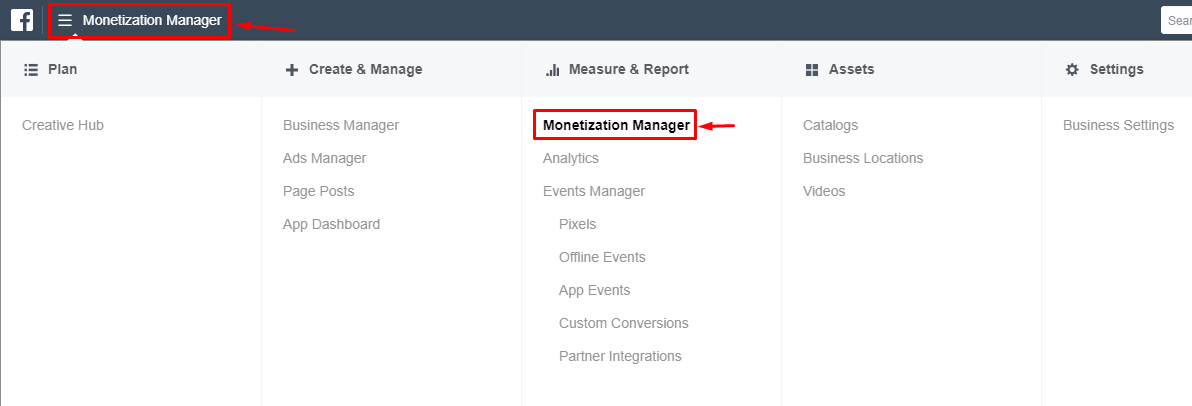
\includegraphics[width = \textwidth]{images/AudienceNetworkEnglish.png}
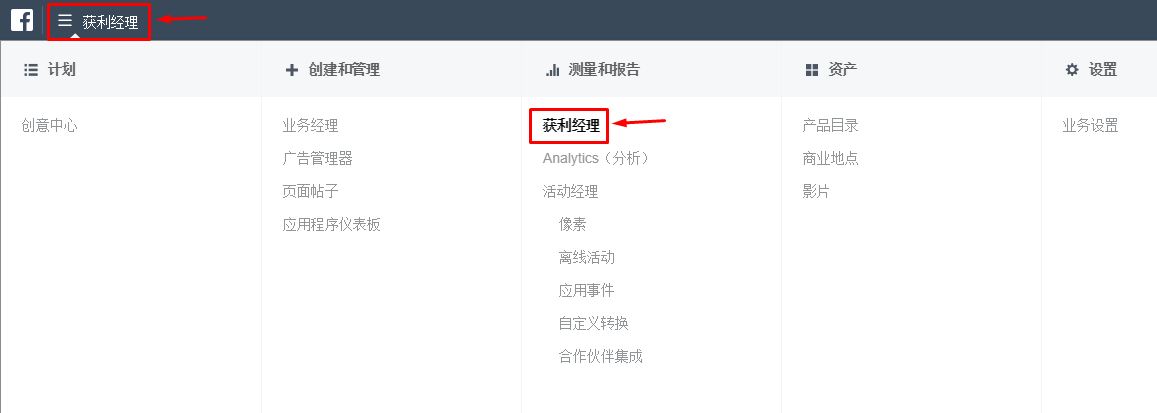
\includegraphics[width = \textwidth]{images/AudienceNetworkChinese.png}
\end{center}

The Audience Network is further split into Property, Platform, and Placement. 

\subsubsection{Property}
This is the highest level of the audience network. A property is the same idea as a product, for instance one game that the company has made. Click on "Create A Property" to add a new product under the Audience Network

\begin{center}
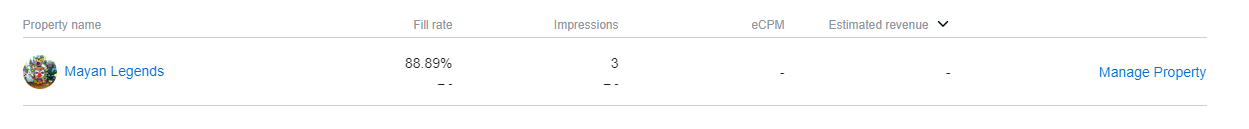
\includegraphics[width = \textwidth]{images/Property.png}
\end{center}

\subsubsection{Platform}
The platform is a sub-level of a property. Under a property, an application can have multiple different types of platforms: Android, Web, iOS, Instant Games. Each of these can have their own settings. For now, just use Instant Games for the HuHuGame platform.

\begin{center}
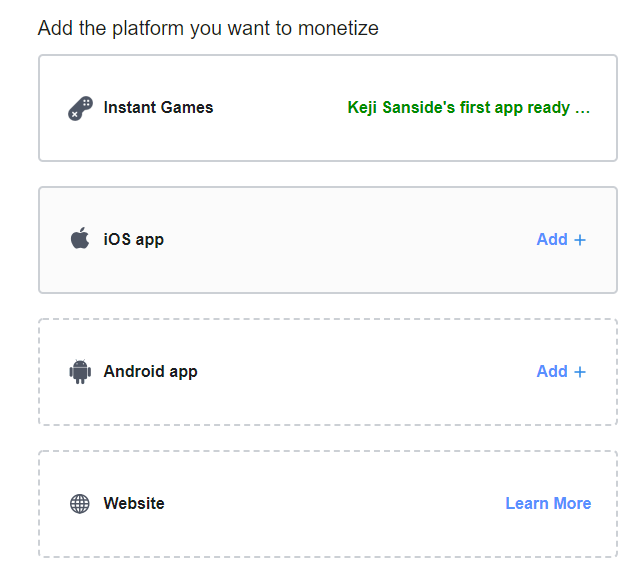
\includegraphics[width = 300px]{images/Platform.png}
\end{center}

\subsubsection{Placement}
A placement is the lowest level of the audience network. It is the same as having a spot to put your advertisement in your application. Each application can have a maximum of 4 different advertisements. For Instant Games, these can be interstitial or video ads. Furthermore, each advertisement is given a unique code which is later necessary for use when adding the code for advertisements to show in the application.

\begin{center}
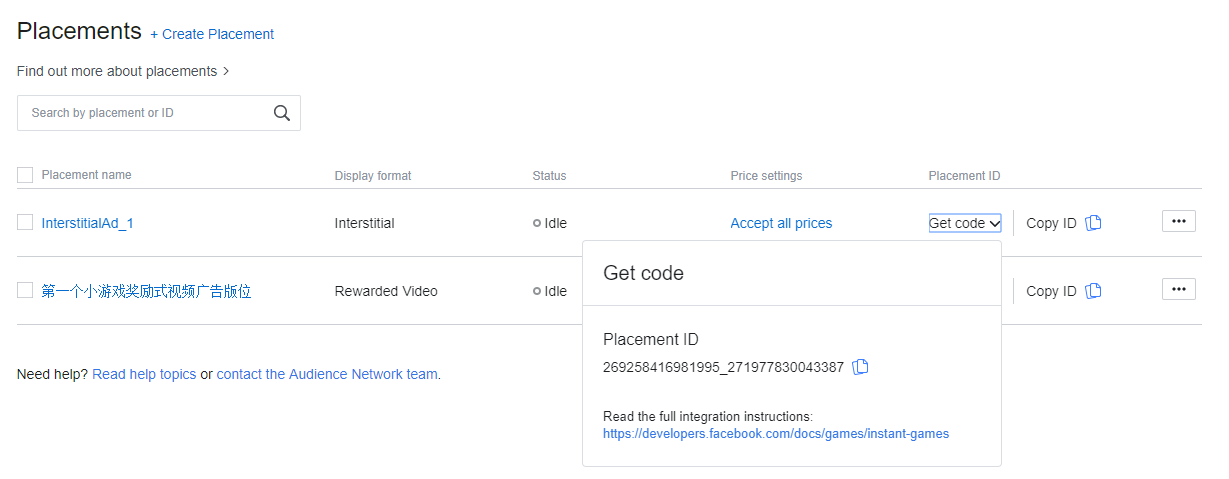
\includegraphics[width = \textwidth]{images/Placements.png}
\end{center}

\subsection{Interstitial and Video Ads}
There are two types of ads that can be added into an Instant Game, interstitial ads and video ads. Each has their own calling functions that are slightly different. Still, each ad can be integrated very easily by using Facebook's integrated functions. The long string of numbers within the FBInstant.getAdAsync() function is a unique number that can be found on the audience network page for each game. Facebook allows for a maximum of 4 different kinds of advertisements within one Instant Game.

\begin{center}
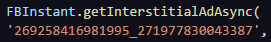
\includegraphics[]{images/UniqueAd.png}
\end{center}

\vspace{.5cm}
\href{https://developers.facebook.com/docs/games/instant-games/sdk/fbinstant6.1#adinstance}{Facebook Instant Games API Advertisements Reference 6.1}

\subsubsection{Interstitial Ads}
Interstitial ads are full page images that appear across the entire device screen.These can be called using the following function:

\begin{center}
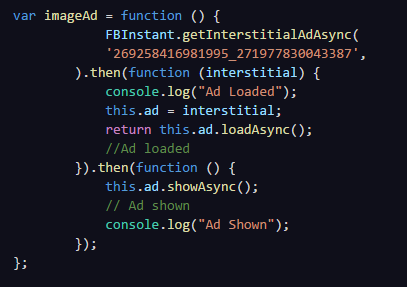
\includegraphics[width = 300px]{images/InterstitialAds.png}
\end{center}

\subsubsection{Video Ads}
Interstitial ads are full page videos that play across the entire device screen. These can be called using the following function. They can also be checked to see if the video was watched through entirely or stopped before completion:

\begin{center}
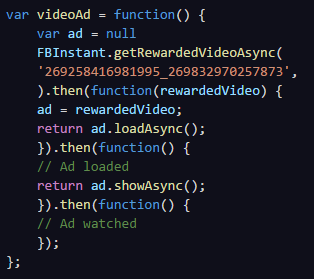
\includegraphics[]{images/VideoAds.png}
\end{center}

\section{Getting Ready for Review}
\subsection{Basic Information}
After creating the application, writing all the code, and implementing advertisements there are multiple different files and items that need to be created before being able to send the application into review. Mostly, this includes linking the privacy policy to the game, as well as, uploading some images and a video to show how the game looks like to users.

\begin{center}
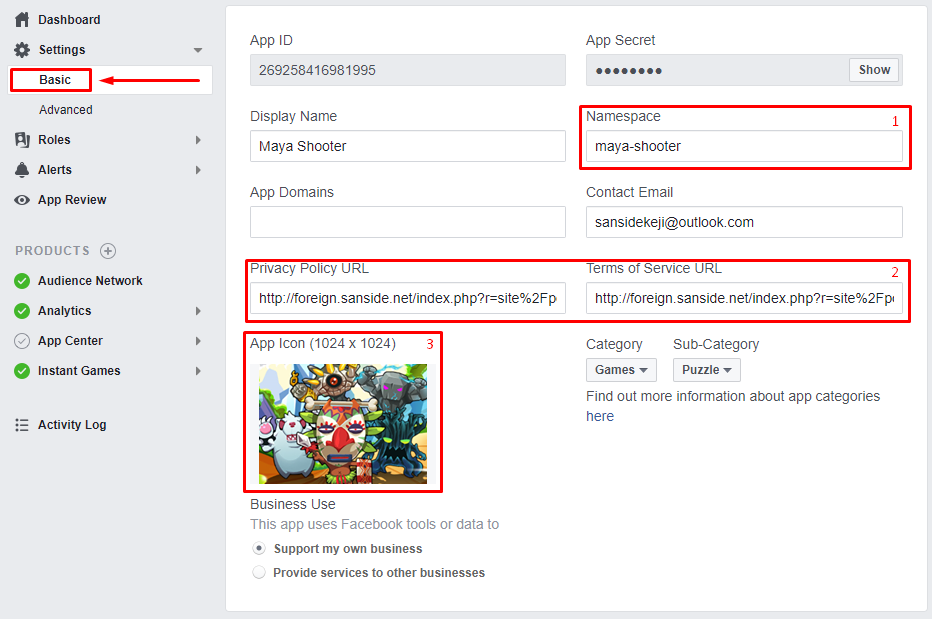
\includegraphics[width=\textwidth]{images/basicinfo.png}
\end{center}

In the above image, the most important steps under the basic tab are described. 
\begin{enumerate}
\item The namespace describes how your game can be found when searching for it. For example, here it is "maya-shooter" and we can find the application by going to "apps.facebook.com/maya-shooter"
\item Privacy Policy and Terms of Service URL links are needed. This will always be: "http://foreign.sanside.net/index.php?r=site\%2Fpolicy" which is the new privacy policy that was translated into english
\item The App Icon is the main picture of the application that you will see when looking for the game. This is the most common icon that will appear for the game. The size is 1024x1024.
\item You should also choose the category of app to be "Game" and change the sub-category based on what kind of game it is.
\end{enumerate}

\subsection{Instant Games Details}
Under the instant games tab, you will have to put more information about the game you are uploading.

\begin{center}
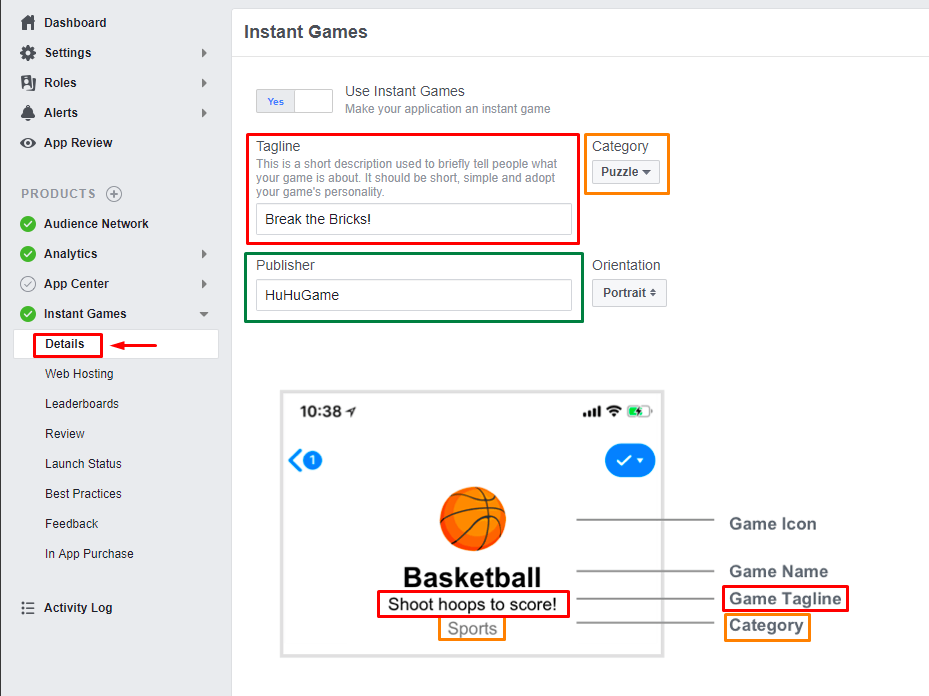
\includegraphics[width=400px]{images/instantdetails1.png}
\end{center}

Under the instant games tab, you will need to give specific information pertaining to the game you created and how it will appear in the application. The following things that need to be added have been color coded to show where they appear. Here you need to:
\begin{itemize}
\item include a tagline, which is similar to a quick slogan about the game. Try to explain the game in less than 10 words. 
\item choose the category that the game is liste under. In this case, Maya Shooter was a puzzle game so I chose puzzle.
\item Write the publisher name. This will be either HuHuGame or Sanside Technology depending on what you would like to put.
\end{itemize}


\begin{center}
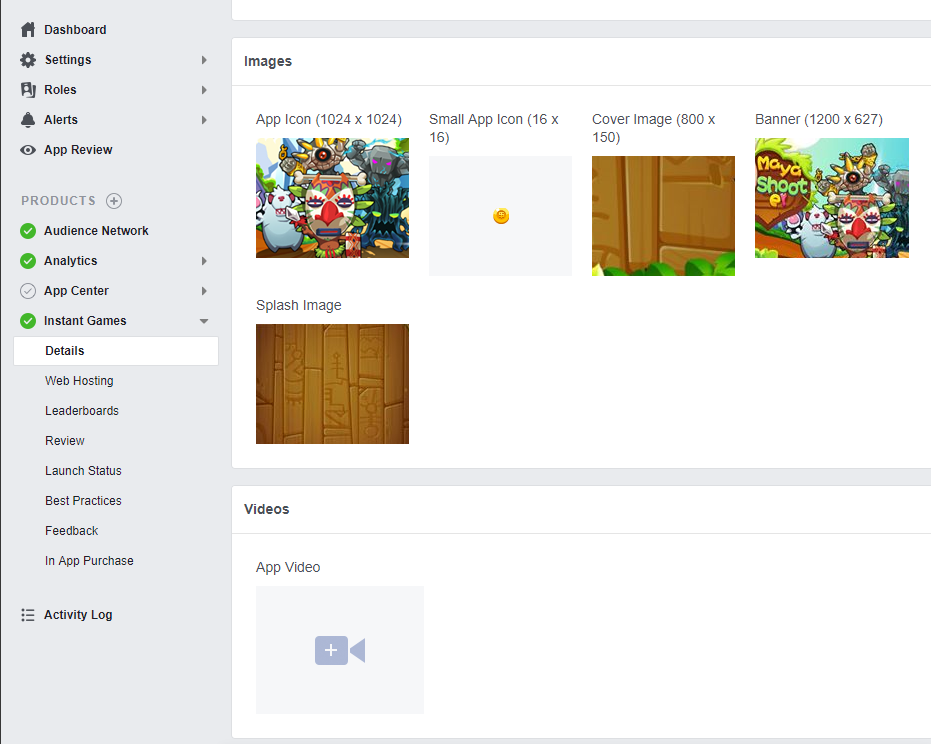
\includegraphics[width=400px]{images/instantdetails2.png}
\end{center}
The following images and video files also have to be uploaded before submitting the game for review. These files are usually used when searching for your game and finding it in the Facebook Instant Games Store. Below is a link to the full article of the App Center Tab and what images need to be uploaded as well as a picture that shows what each of the pictures will be used for. 

The splash image is not listed, but it is the background of the game while it is loading. I have been using the game backgrounds (without the logo or characters) as the splash screen as it fits well with what a splash screen is suppose to be.

\hyperlink{https://developers.facebook.com/docs/games/listing/}{App Center Tab Explained Here}

\begin{center}
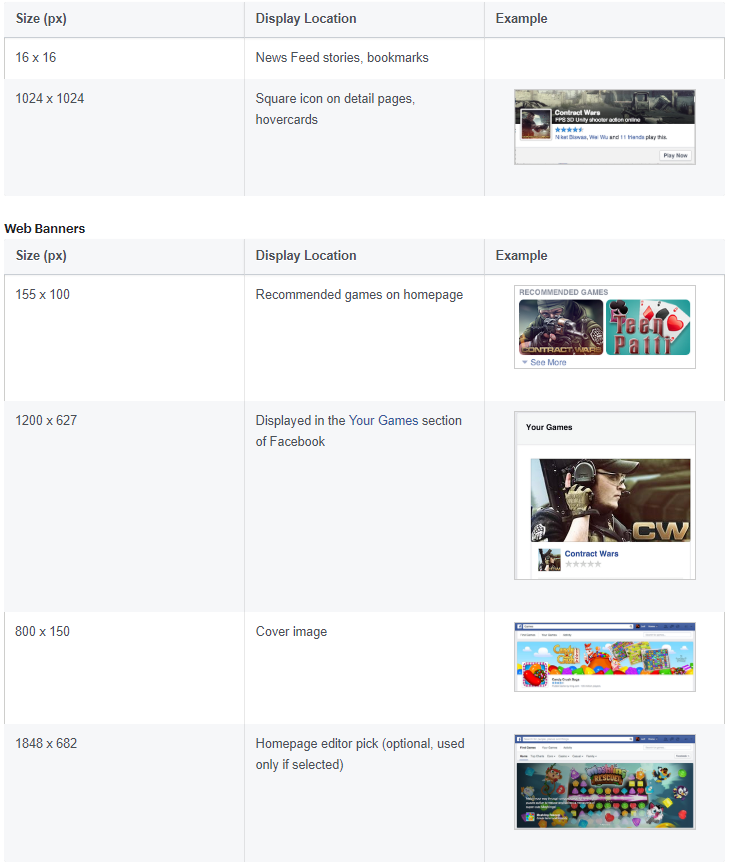
\includegraphics[width=\textwidth]{images/picturesexplained.png}
\end{center}

\subsection{Creating an App Page}
In order to promote the game as well as let other people know about information that is coming out about the game or any news with updates, each facebook application should be linked to a facebook app page. This is similar to a facebook profile, except that it is specifically for the game instead of a facebook person like a normal facebook page is for.

\begin{center}
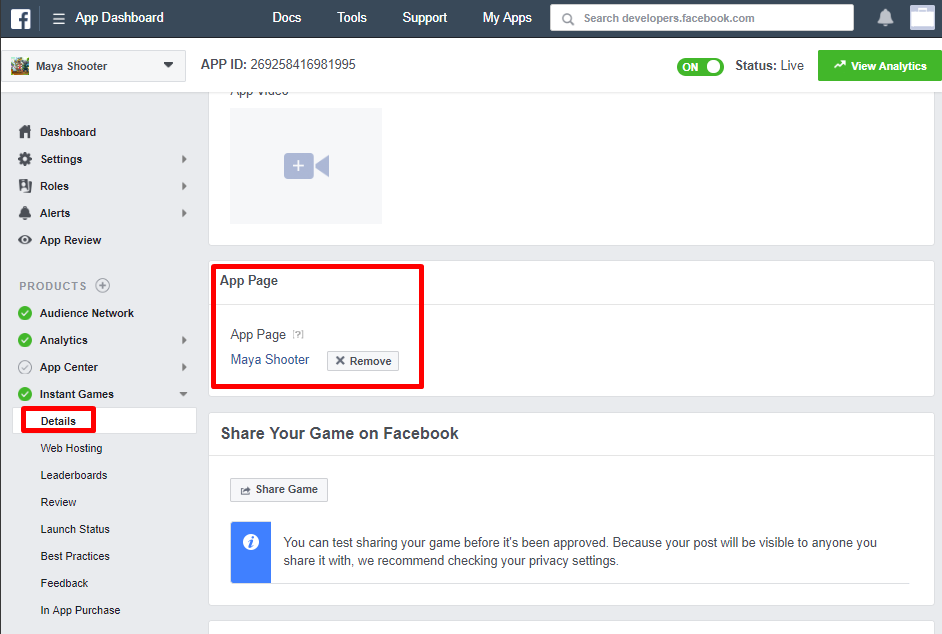
\includegraphics[width=\textwidth]{images/apppage.png}
\end{center}

When making a new app page, the following image above will be different, asking instead to create a page. When creating a page, click on the Business side on the left and under category choose "App Page". Finally, name it same as the name of the application so that it is easy to see what the page is for.You can customize this page more to market your game and try to post pictures, events or information about the game here to get more players to play the game. You can also make a button that gets players to play. I recommend just looking at all the features on the page, as there are too many to explain thoroughly.

\section{Sending for Review}
After the game is integrated with the Facebook SDK, Advertisements are implemented with Audience Network, and all the necessary information is posted, you can apply for a review process by Facebook to finally get the game onto Facebook.com. 

\begin{enumerate}
\item First, go to the App Review tab and switch the button to make your application go live. This will allow confirm that your application is allowed to be used on Facebook.com

Note: At one point in the process of the review, you will be asked to provide the Apple developer team ID. You can either log into developer.apple.com website and find it, or use it from the image below:

\begin{center}
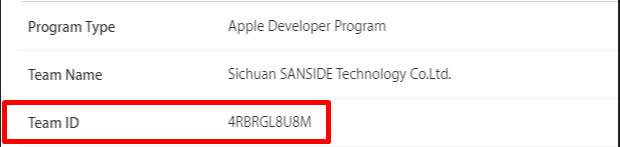
\includegraphics[width=300px]{images/apple.png}
\end{center}

\begin{center}
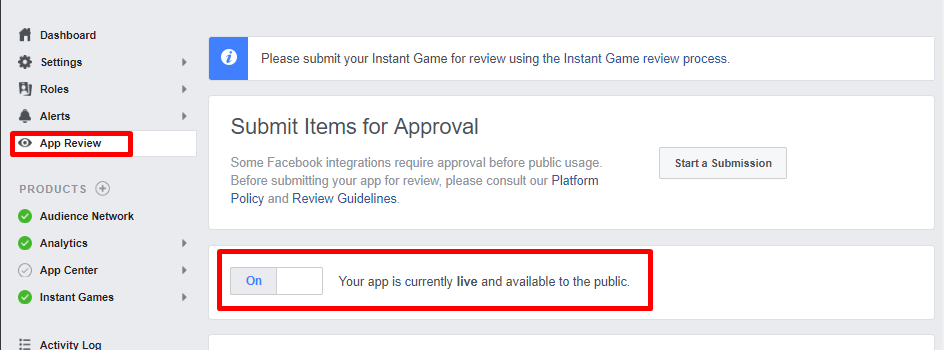
\includegraphics[width=\textwidth]{images/appreview.png}
\end{center}
\item Then, we also need to submit the instant game part of the game for review. Under the Instant Games tab click review and select "Add to Submission" near "Instant Game". If your game also has in app purchases, then the other one will have to be selected as well. 
\begin{center}
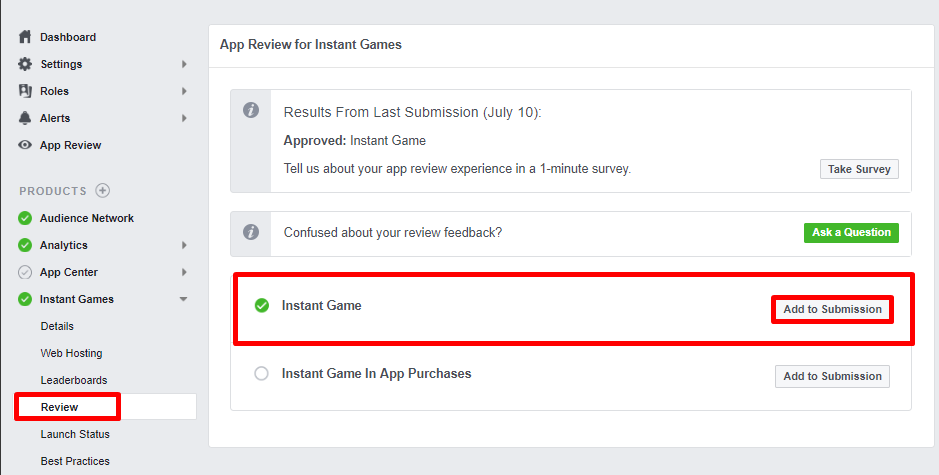
\includegraphics[width=\textwidth]{images/instantreview.png}
\end{center}
\item This part of the process takes the longest time of waiting. After submitting both reviews, you will need to wait for Facebook to accept them and get back to you. If they accept, then you are clear to go onto the next step and launch the game; if not, then see what they say you did incorrectly, change it, and send it for submission again.
\end{enumerate}
\section{Launch Status}
Finally, after doing everything else, you are ready to launch. If you do not know if you did everything, you will be ready to launch if the Game Review icon on the left side (seen below) has a green checkmark. If not, go to the review and see what you are missing before continuing.

\begin{center}
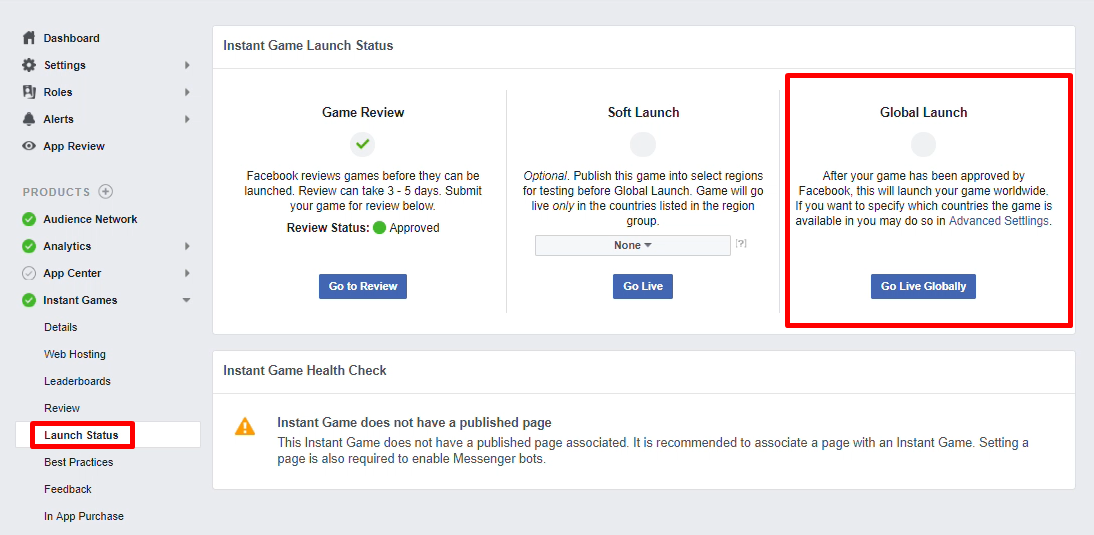
\includegraphics[width=\textwidth]{images/launch.png}
\end{center}

Press "Go Live Globally" to launch the game to the rest of the world! 

Note: You can only globally launch an app, once a week. If you are trying to put a lot of games onto Facebook, you will only be able to do one every 7 days.
\vfill{}

\begin{center}

\includegraphics[width=\textwidth]{images/congratulations.jpg}
\end{center}



\end{document}